\documentclass{article}

\usepackage{hyperref}
\usepackage{amsmath}
\usepackage{graphicx}
\usepackage{subcaption}
\usepackage{epstopdf}
\usepackage{color}

\usepackage{times}
\usepackage{bm}

% Page layout
\hoffset -0in
\voffset -1in
\oddsidemargin 0in
\textheight 9.3in
\textwidth 6.3in

\setlength{\parindent}{0pt}
%\setlength{\intextsep}{10pt}
%\pagestyle{empty}

\graphicspath{{figures/}}

\begin{document}
	\section*{COMPUTATIONAL METHODS IN MECHANICS: Assignment 7}
	Vesa-Ville Hurskainen, 21 Mar 2018\\
	\href{https://github.com/VesaVilleHurskainen/cmim2018}{GitHub repository}

	\section*{Introduction}
	This is a report of the seventh assignment of the course \textit{Computational Methods in Mechanics}. The assignment consists of three tasks, which are as follows:
	\begin{enumerate}
		\setlength\itemsep{0pt}
		\item To write a general software that can perform kinematic analysis.
		\item To solve a four-bar linkage using the software.
		\item To compare the results with an MBD package, e.g. MSC ADAMS.
	\end{enumerate}

	\section*{Methods}
	The program was written in MATLAB. It is operated via an input file, in which the parameters are defined and the main solution functions are called. For the four-bar example, input was defined in the file~\texttt{inputData.m}. For kinematic solution, the bodies as well as their constraints (joints and rheonomic constraints) should be defined here. In the current program, all data is saved in a MATLAB struct for passing into subprograms. It is structured as follows:\\
	
	\texttt{data} (struct):
	\vspace{-1ex}
	\begin{itemize}
		\setlength\itemsep{0pt}
		\item \texttt{timespan} (vector)
		\item \texttt{bodies} (struct array)
		\vspace{-1ex}
		\begin{itemize}
			\setlength\itemsep{0pt}
			\item \texttt{body} (struct):\quad \texttt{type}, \texttt{position}, \texttt{length}
		\end{itemize}
		\item \texttt{joints}
		\vspace{-1ex}
		\begin{itemize}
			\setlength\itemsep{0pt}
			\item \texttt{joint} (struct):\quad \texttt{type}, \texttt{bodies}, \texttt{positions}
		\end{itemize}
		\item \texttt{constraints}
		\vspace{-1ex}
		\begin{itemize}
			\setlength\itemsep{0pt}
			\item \texttt{constraint} (struct):\quad \texttt{body}, \texttt{dof}, \texttt{expression}, \texttt{diff}, \texttt{ddiff}
		\end{itemize}
	\end{itemize}
	
	The kinematic solution is performed using the function~\texttt{run\_kinematics}, which in turn calls several sub-functions, i.e. for constructing the constraint vector. The program uses the Newton-Raphson method to solve the position, velocity and acceleration equations at each time step. For this computation, Jacobians are computed using the finite difference method. The function~\texttt{pproc\_animate} was written for simplified visualization of the results.\\
	
	The program was employed to solve a four-bar linkage system with the geometry and parameters presented in Figure~\ref*{fig:system}. The results were compared with those computed using ADAMS.
	
	\begin{figure}[htb]
		\centering
		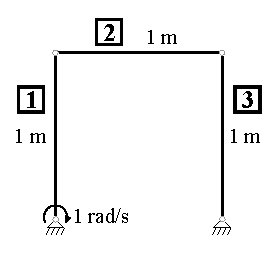
\includegraphics[width=0.25\textwidth]{system.eps}
		\caption{Four-bar system geometry and parameters.\label{fig:system}}
	\end{figure}

	\section*{Results}
	In Figures \ref*{fig:pos}, \ref*{fig:vel} and \ref*{fig:acc}, the errors of position, velocity and acceleration of body 3 (see Fig.~\ref{fig:system}) are presented. The reference results were computed with ADAMS. In all simulations, a time step of $ \Delta t = 10$ ms was used, and the total simulation time was $1$ s.
	
	\vspace{-2ex}
	\begin{figure}[htb]
		\centering
		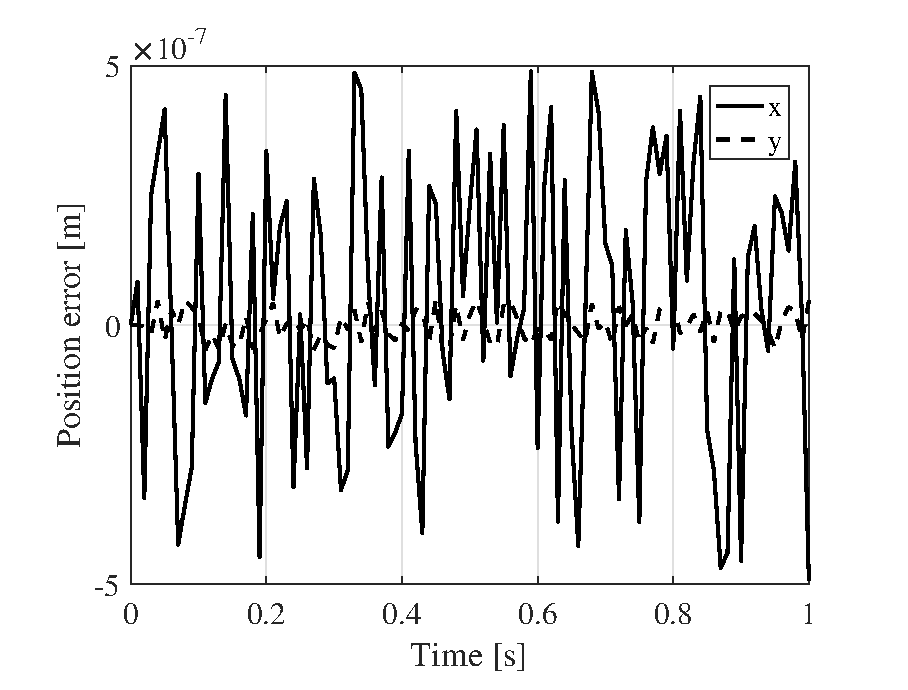
\includegraphics[width=0.4\textwidth]{position.eps}
		\caption{Position error of body 3 in directions x and y, reference values computed using ANSYS.\label{fig:pos}}
	\end{figure}
	\vspace{-2ex}
	\begin{figure}[htb]
		\centering
		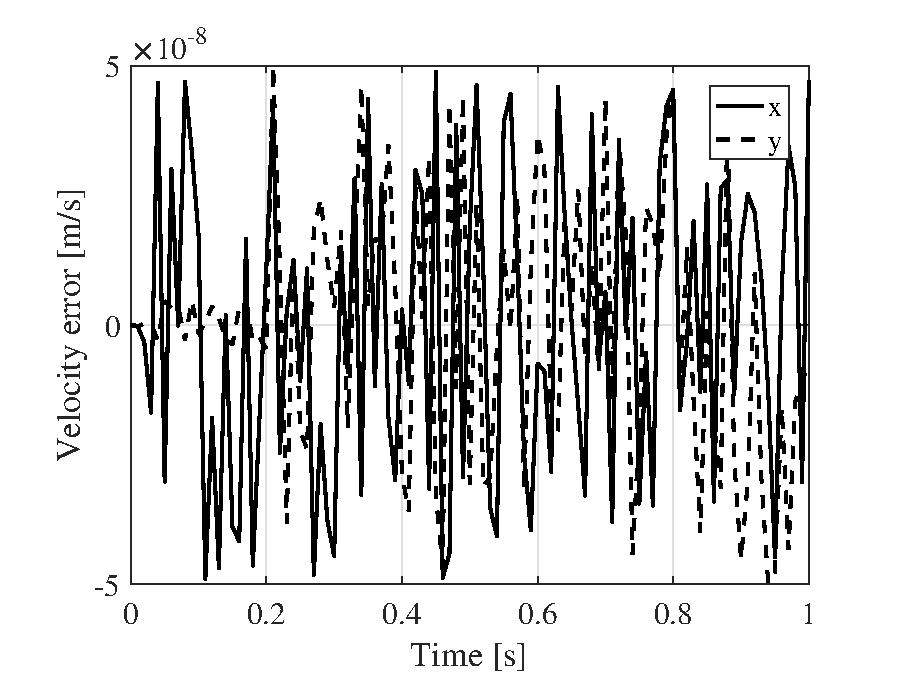
\includegraphics[width=0.4\textwidth]{velocity.eps}
		\caption{Velocity error of body 3 in directions x and y, reference values computed using ANSYS.\label{fig:vel}}
	\end{figure}
	\vspace{-2ex}
	\begin{figure}[htb]
		\centering
		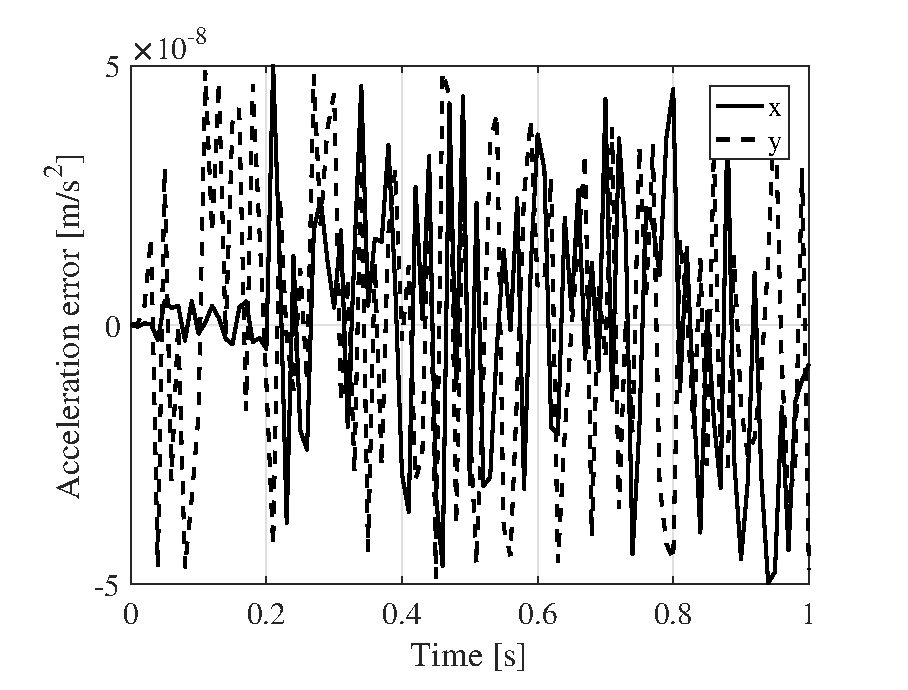
\includegraphics[width=0.4\textwidth]{acceleration.eps}
		\caption{Acceleration error of body 3 in directions x and y, reference values computed using ANSYS.\label{fig:acc}}
	\end{figure}
	
	\section*{Analysis}
	As Figures \ref*{fig:pos}, \ref*{fig:vel} and \ref*{fig:acc} show, the results were in good agreement with ADAMS in the case of the four-bar system, as the errors are very small for all three quantities. However, there is still much room for improvement in the program. For example, only revolute joints and very simple time-dependent constraints are currently implemented. In the same vein, only slender rods are currently implemented as bodies. Additionally, the program's versatility is not known, since it has not yet been tested in many other scenarios.

\end{document}